\documentclass[1p]{elsarticle_modified}
%\bibliographystyle{elsarticle-num}

%\usepackage[colorlinks]{hyperref}
%\usepackage{abbrmath_seonhwa} %\Abb, \Ascr, \Acal ,\Abf, \Afrak
\usepackage{amsfonts}
\usepackage{amssymb}
\usepackage{amsmath}
\usepackage{amsthm}
\usepackage{scalefnt}
\usepackage{amsbsy}
\usepackage{kotex}
\usepackage{caption}
\usepackage{subfig}
\usepackage{color}
\usepackage{graphicx}
\usepackage{xcolor} %% white, black, red, green, blue, cyan, magenta, yellow
\usepackage{float}
\usepackage{setspace}
\usepackage{hyperref}

\usepackage{tikz}
\usetikzlibrary{arrows}

\usepackage{multirow}
\usepackage{array} % fixed length table
\usepackage{hhline}

%%%%%%%%%%%%%%%%%%%%%
\makeatletter
\renewcommand*\env@matrix[1][\arraystretch]{%
	\edef\arraystretch{#1}%
	\hskip -\arraycolsep
	\let\@ifnextchar\new@ifnextchar
	\array{*\c@MaxMatrixCols c}}
\makeatother %https://tex.stackexchange.com/questions/14071/how-can-i-increase-the-line-spacing-in-a-matrix
%%%%%%%%%%%%%%%

\usepackage[normalem]{ulem}

\newcommand{\msout}[1]{\ifmmode\text{\sout{\ensuremath{#1}}}\else\sout{#1}\fi}
%SOURCE: \msout is \stkout macro in https://tex.stackexchange.com/questions/20609/strikeout-in-math-mode

\newcommand{\cancel}[1]{
	\ifmmode
	{\color{red}\msout{#1}}
	\else
	{\color{red}\sout{#1}}
	\fi
}

\newcommand{\add}[1]{
	{\color{blue}\uwave{#1}}
}

\newcommand{\replace}[2]{
	\ifmmode
	{\color{red}\msout{#1}}{\color{blue}\uwave{#2}}
	\else
	{\color{red}\sout{#1}}{\color{blue}\uwave{#2}}
	\fi
}

\newcommand{\Sol}{\mathcal{S}} %segment
\newcommand{\D}{D} %diagram
\newcommand{\A}{\mathcal{A}} %arc


%%%%%%%%%%%%%%%%%%%%%%%%%%%%%5 test

\def\sl{\operatorname{\textup{SL}}(2,\Cbb)}
\def\psl{\operatorname{\textup{PSL}}(2,\Cbb)}
\def\quan{\mkern 1mu \triangleright \mkern 1mu}

\theoremstyle{definition}
\newtheorem{thm}{Theorem}[section]
\newtheorem{prop}[thm]{Proposition}
\newtheorem{lem}[thm]{Lemma}
\newtheorem{ques}[thm]{Question}
\newtheorem{cor}[thm]{Corollary}
\newtheorem{defn}[thm]{Definition}
\newtheorem{exam}[thm]{Example}
\newtheorem{rmk}[thm]{Remark}
\newtheorem{alg}[thm]{Algorithm}

\newcommand{\I}{\sqrt{-1}}
\begin{document}

%\begin{frontmatter}
%
%\title{Boundary parabolic representations of knots up to 8 crossings}
%
%%% Group authors per affiliation:
%\author{Yunhi Cho} 
%\address{Department of Mathematics, University of Seoul, Seoul, Korea}
%\ead{yhcho@uos.ac.kr}
%
%
%\author{Seonhwa Kim} %\fnref{s_kim}}
%\address{Center for Geometry and Physics, Institute for Basic Science, Pohang, 37673, Korea}
%\ead{ryeona17@ibs.re.kr}
%
%\author{Hyuk Kim}
%\address{Department of Mathematical Sciences, Seoul National University, Seoul 08826, Korea}
%\ead{hyukkim@snu.ac.kr}
%
%\author{Seokbeom Yoon}
%\address{Department of Mathematical Sciences, Seoul National University, Seoul, 08826,  Korea}
%\ead{sbyoon15@snu.ac.kr}
%
%\begin{abstract}
%We find all boundary parabolic representation of knots up to 8 crossings.
%
%\end{abstract}
%\begin{keyword}
%    \MSC[2010] 57M25 
%\end{keyword}
%
%\end{frontmatter}

%\linenumbers
%\tableofcontents
%
\newcommand\colored[1]{\textcolor{white}{\rule[-0.35ex]{0.8em}{1.4ex}}\kern-0.8em\color{red} #1}%
%\newcommand\colored[1]{\textcolor{white}{ #1}\kern-2.17ex	\textcolor{white}{ #1}\kern-1.81ex	\textcolor{white}{ #1}\kern-2.15ex\color{red}#1	}

{\Large $\underline{12a_{0729}~(K12a_{0729})}$}

\setlength{\tabcolsep}{10pt}
\renewcommand{\arraystretch}{1.6}
\vspace{1cm}\begin{tabular}{m{100pt}>{\centering\arraybackslash}m{274pt}}
\multirow{5}{120pt}{
	\centering
	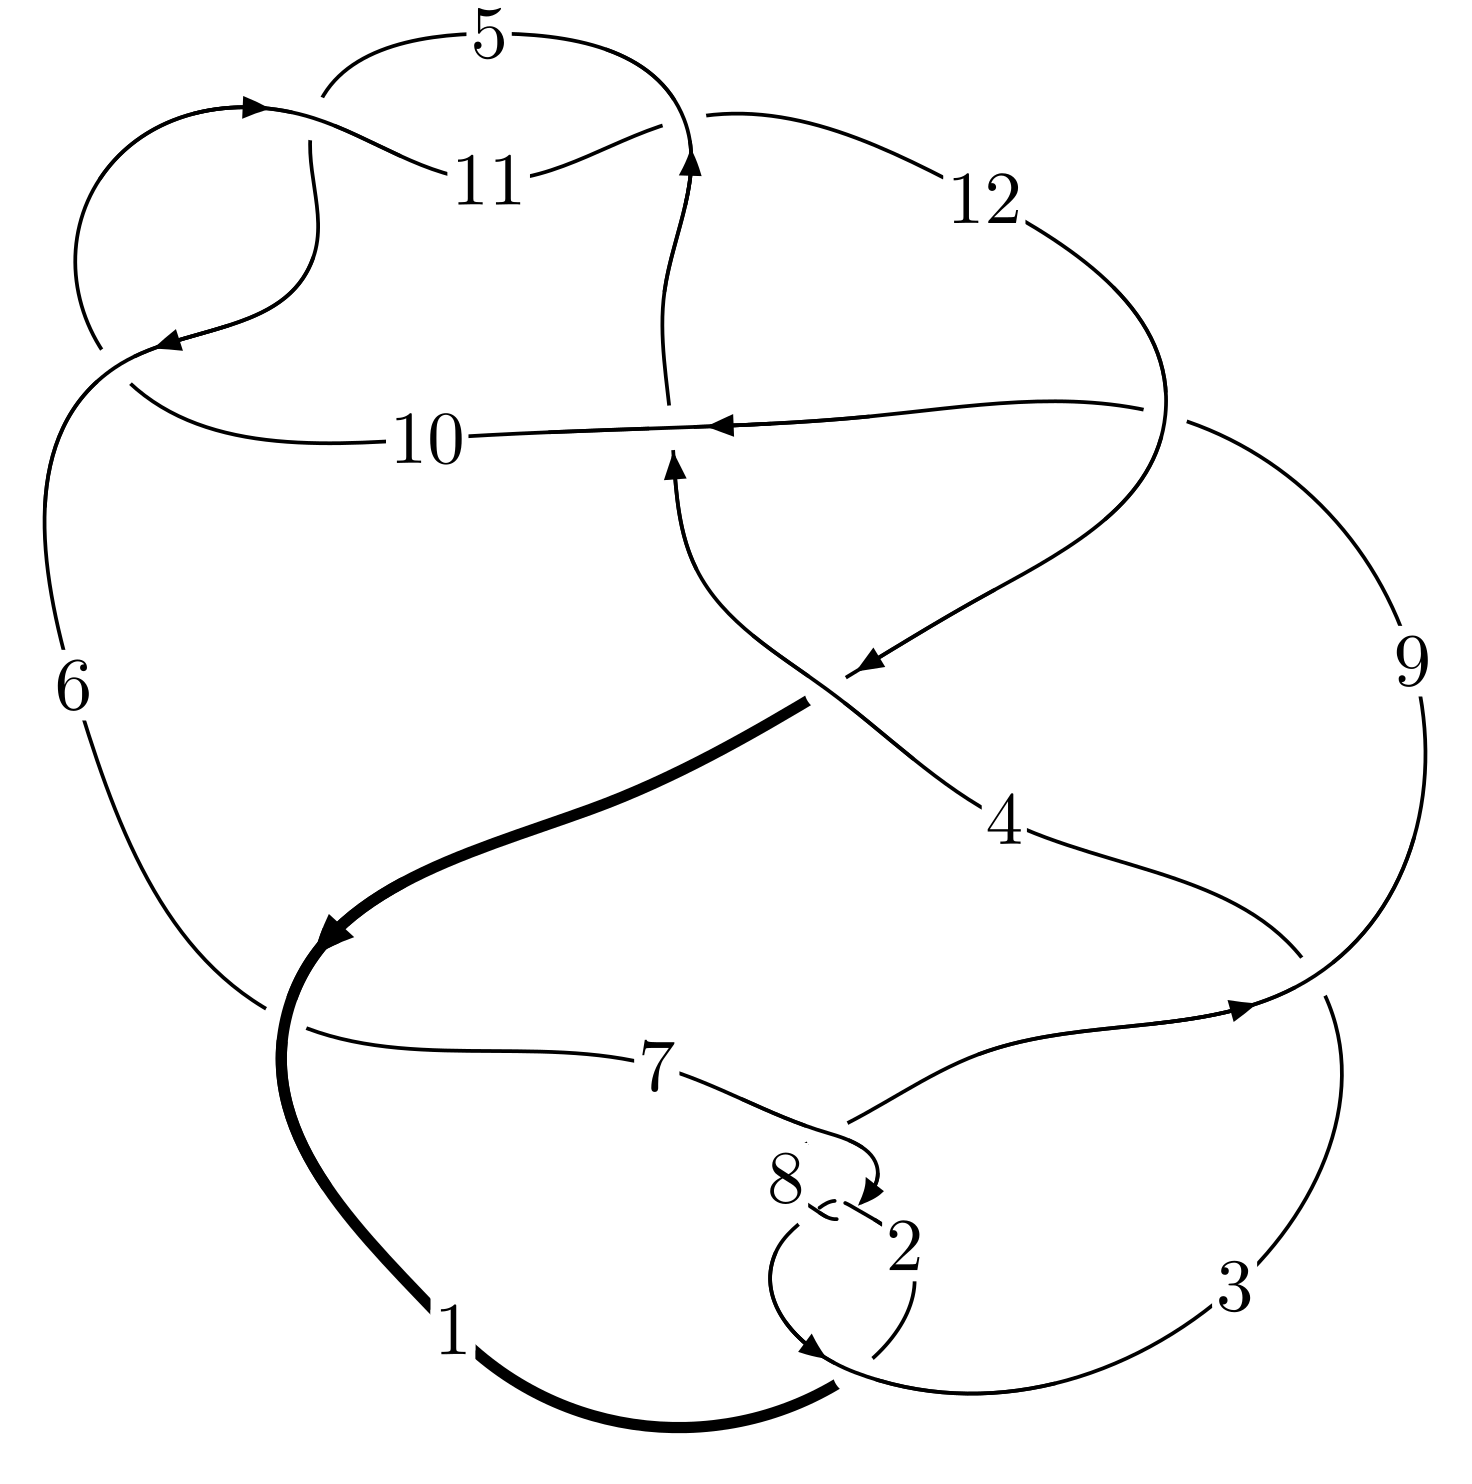
\includegraphics[width=112pt]{../../../GIT/diagram.site/Diagrams/png/1530_12a_0729.png}\\
\ \ \ A knot diagram\footnotemark}&
\allowdisplaybreaks
\textbf{Linearized knot diagam} \\
\cline{2-2}
 &
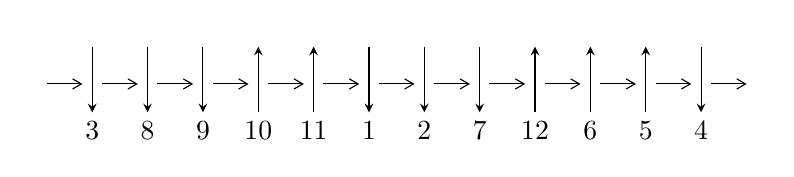
\begin{tikzpicture}[x=20pt, y=17pt]
	% nodes
	\node (C0) at (0, 0) {};
	\node (C1) at (1, 0) {};
	\node (C1U) at (1, +1) {};
	\node (C1D) at (1, -1) {3};

	\node (C2) at (2, 0) {};
	\node (C2U) at (2, +1) {};
	\node (C2D) at (2, -1) {8};

	\node (C3) at (3, 0) {};
	\node (C3U) at (3, +1) {};
	\node (C3D) at (3, -1) {9};

	\node (C4) at (4, 0) {};
	\node (C4U) at (4, +1) {};
	\node (C4D) at (4, -1) {10};

	\node (C5) at (5, 0) {};
	\node (C5U) at (5, +1) {};
	\node (C5D) at (5, -1) {11};

	\node (C6) at (6, 0) {};
	\node (C6U) at (6, +1) {};
	\node (C6D) at (6, -1) {1};

	\node (C7) at (7, 0) {};
	\node (C7U) at (7, +1) {};
	\node (C7D) at (7, -1) {2};

	\node (C8) at (8, 0) {};
	\node (C8U) at (8, +1) {};
	\node (C8D) at (8, -1) {7};

	\node (C9) at (9, 0) {};
	\node (C9U) at (9, +1) {};
	\node (C9D) at (9, -1) {12};

	\node (C10) at (10, 0) {};
	\node (C10U) at (10, +1) {};
	\node (C10D) at (10, -1) {6};

	\node (C11) at (11, 0) {};
	\node (C11U) at (11, +1) {};
	\node (C11D) at (11, -1) {5};

	\node (C12) at (12, 0) {};
	\node (C12U) at (12, +1) {};
	\node (C12D) at (12, -1) {4};
	\node (C13) at (13, 0) {};

	% arrows
	\draw[->,>={angle 60}]
	(C0) edge (C1) (C1) edge (C2) (C2) edge (C3) (C3) edge (C4) (C4) edge (C5) (C5) edge (C6) (C6) edge (C7) (C7) edge (C8) (C8) edge (C9) (C9) edge (C10) (C10) edge (C11) (C11) edge (C12) (C12) edge (C13) ;	\draw[->,>=stealth]
	(C1U) edge (C1D) (C2U) edge (C2D) (C3U) edge (C3D) (C4D) edge (C4U) (C5D) edge (C5U) (C6U) edge (C6D) (C7U) edge (C7D) (C8U) edge (C8D) (C9D) edge (C9U) (C10D) edge (C10U) (C11D) edge (C11U) (C12U) edge (C12D) ;
	\end{tikzpicture} \\
\hhline{~~} \\& 
\textbf{Solving Sequence} \\ \cline{2-2} 
 &
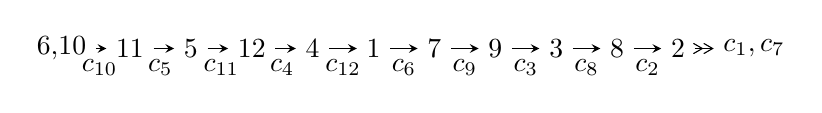
\begin{tikzpicture}[x=22pt, y=7pt]
	% node
	\node (A0) at (-1/8, 0) {6,10};
	\node (A1) at (1, 0) {11};
	\node (A2) at (2, 0) {5};
	\node (A3) at (3, 0) {12};
	\node (A4) at (4, 0) {4};
	\node (A5) at (5, 0) {1};
	\node (A6) at (6, 0) {7};
	\node (A7) at (7, 0) {9};
	\node (A8) at (8, 0) {3};
	\node (A9) at (9, 0) {8};
	\node (A10) at (10, 0) {2};
	\node (C1) at (1/2, -1) {$c_{10}$};
	\node (C2) at (3/2, -1) {$c_{5}$};
	\node (C3) at (5/2, -1) {$c_{11}$};
	\node (C4) at (7/2, -1) {$c_{4}$};
	\node (C5) at (9/2, -1) {$c_{12}$};
	\node (C6) at (11/2, -1) {$c_{6}$};
	\node (C7) at (13/2, -1) {$c_{9}$};
	\node (C8) at (15/2, -1) {$c_{3}$};
	\node (C9) at (17/2, -1) {$c_{8}$};
	\node (C10) at (19/2, -1) {$c_{2}$};
	\node (A11) at (45/4, 0) {$c_{1},c_{7}$};

	% edge
	\draw[->,>=stealth]	
	(A0) edge (A1) (A1) edge (A2) (A2) edge (A3) (A3) edge (A4) (A4) edge (A5) (A5) edge (A6) (A6) edge (A7) (A7) edge (A8) (A8) edge (A9) (A9) edge (A10) ;
	\draw[->>,>={angle 60}]	
	(A10) edge (A11);
\end{tikzpicture} \\ 

\end{tabular} \\

\footnotetext{
The image of knot diagram is generated by the software ``\textbf{Draw programme}" developed by Andrew Bartholomew(\url{http://www.layer8.co.uk/maths/draw/index.htm\#Running-draw}), where we modified some parts for our purpose(\url{https://github.com/CATsTAILs/LinksPainter}).
}\phantom \\ \newline 
\centering \textbf{Ideals for irreducible components\footnotemark of $X_{\text{par}}$} 
 
\begin{align*}
I^u_{1}&=\langle 
u^{83}+u^{82}+\cdots+u^2-1\rangle \\
\\
\end{align*}
\raggedright * 1 irreducible components of $\dim_{\mathbb{C}}=0$, with total 83 representations.\\
\footnotetext{All coefficients of polynomials are rational numbers. But the coefficients are sometimes approximated in decimal forms when there is not enough margin.}
\newpage
\renewcommand{\arraystretch}{1}
\centering \section*{I. $I^u_{1}= \langle u^{83}+u^{82}+\cdots+u^2-1 \rangle$}
\flushleft \textbf{(i) Arc colorings}\\
\begin{tabular}{m{7pt} m{180pt} m{7pt} m{180pt} }
\flushright $a_{6}=$&$\begin{pmatrix}0\\u\end{pmatrix}$ \\
\flushright $a_{10}=$&$\begin{pmatrix}1\\0\end{pmatrix}$ \\
\flushright $a_{11}=$&$\begin{pmatrix}1\\- u^2\end{pmatrix}$ \\
\flushright $a_{5}=$&$\begin{pmatrix}- u\\u^3+u\end{pmatrix}$ \\
\flushright $a_{12}=$&$\begin{pmatrix}u^2+1\\- u^4-2 u^2\end{pmatrix}$ \\
\flushright $a_{4}=$&$\begin{pmatrix}- u^3-2 u\\u^3+u\end{pmatrix}$ \\
\flushright $a_{1}=$&$\begin{pmatrix}u^{10}+5 u^8+8 u^6+3 u^4- u^2+1\\- u^{10}-4 u^8-5 u^6-2 u^4- u^2\end{pmatrix}$ \\
\flushright $a_{7}=$&$\begin{pmatrix}- u^{21}-10 u^{19}+\cdots+2 u^3- u\\u^{21}+9 u^{19}+33 u^{17}+62 u^{15}+62 u^{13}+33 u^{11}+13 u^9+6 u^7+u^5+u^3+u\end{pmatrix}$ \\
\flushright $a_{9}=$&$\begin{pmatrix}- u^6-3 u^4-2 u^2+1\\u^8+4 u^6+4 u^4\end{pmatrix}$ \\
\flushright $a_{3}=$&$\begin{pmatrix}- u^{17}-8 u^{15}-25 u^{13}-36 u^{11}-19 u^9+4 u^7+2 u^5-4 u^3- u\\u^{19}+9 u^{17}+32 u^{15}+55 u^{13}+43 u^{11}+9 u^9+4 u^5+u^3+u\end{pmatrix}$ \\
\flushright $a_{8}=$&$\begin{pmatrix}u^{50}+23 u^{48}+\cdots- u^2+1\\- u^{50}-22 u^{48}+\cdots+4 u^4- u^2\end{pmatrix}$ \\
\flushright $a_{2}=$&$\begin{pmatrix}- u^{46}-21 u^{44}+\cdots-2 u^2+1\\u^{48}+22 u^{46}+\cdots-2 u^6-2 u^4\end{pmatrix}$\\&\end{tabular}
\flushleft \textbf{(ii) Obstruction class $= -1$}\\~\\
\flushleft \textbf{(iii) Cusp Shapes $= -4 u^{82}-4 u^{81}+\cdots-4 u-2$}\\~\\
\newpage\renewcommand{\arraystretch}{1}
\flushleft \textbf{(iv) u-Polynomials at the component}\newline \\
\begin{tabular}{m{50pt}|m{274pt}}
Crossings & \hspace{64pt}u-Polynomials at each crossing \\
\hline $$\begin{aligned}c_{1},c_{8}\end{aligned}$$&$\begin{aligned}
&u^{83}+29 u^{82}+\cdots+2 u+1
\end{aligned}$\\
\hline $$\begin{aligned}c_{2},c_{7}\end{aligned}$$&$\begin{aligned}
&u^{83}+u^{82}+\cdots+2 u+1
\end{aligned}$\\
\hline $$\begin{aligned}c_{3},c_{6}\end{aligned}$$&$\begin{aligned}
&u^{83}- u^{82}+\cdots-134 u+61
\end{aligned}$\\
\hline $$\begin{aligned}c_{4}\end{aligned}$$&$\begin{aligned}
&u^{83}+u^{82}+\cdots+12 u+1
\end{aligned}$\\
\hline $$\begin{aligned}c_{5},c_{10},c_{11}\end{aligned}$$&$\begin{aligned}
&u^{83}- u^{82}+\cdots- u^2+1
\end{aligned}$\\
\hline $$\begin{aligned}c_{9}\end{aligned}$$&$\begin{aligned}
&u^{83}+17 u^{82}+\cdots-49616 u-2993
\end{aligned}$\\
\hline $$\begin{aligned}c_{12}\end{aligned}$$&$\begin{aligned}
&u^{83}-7 u^{82}+\cdots+24 u-1
\end{aligned}$\\
\hline
\end{tabular}\\~\\
\newpage\renewcommand{\arraystretch}{1}
\flushleft \textbf{(v) Riley Polynomials at the component}\newline \\
\begin{tabular}{m{50pt}|m{274pt}}
Crossings & \hspace{64pt}Riley Polynomials at each crossing \\
\hline $$\begin{aligned}c_{1},c_{8}\end{aligned}$$&$\begin{aligned}
&y^{83}+51 y^{82}+\cdots-14 y-1
\end{aligned}$\\
\hline $$\begin{aligned}c_{2},c_{7}\end{aligned}$$&$\begin{aligned}
&y^{83}-29 y^{82}+\cdots+2 y-1
\end{aligned}$\\
\hline $$\begin{aligned}c_{3},c_{6}\end{aligned}$$&$\begin{aligned}
&y^{83}-57 y^{82}+\cdots+104454 y-3721
\end{aligned}$\\
\hline $$\begin{aligned}c_{4}\end{aligned}$$&$\begin{aligned}
&y^{83}+7 y^{82}+\cdots-46 y-1
\end{aligned}$\\
\hline $$\begin{aligned}c_{5},c_{10},c_{11}\end{aligned}$$&$\begin{aligned}
&y^{83}+75 y^{82}+\cdots+2 y-1
\end{aligned}$\\
\hline $$\begin{aligned}c_{9}\end{aligned}$$&$\begin{aligned}
&y^{83}+31 y^{82}+\cdots-117757622 y-8958049
\end{aligned}$\\
\hline $$\begin{aligned}c_{12}\end{aligned}$$&$\begin{aligned}
&y^{83}- y^{82}+\cdots-70 y-1
\end{aligned}$\\
\hline
\end{tabular}\\~\\
\newpage\flushleft \textbf{(vi) Complex Volumes and Cusp Shapes}
$$\begin{array}{c|c|c}  
\text{Solutions to }I^u_{1}& \I (\text{vol} + \sqrt{-1}CS) & \text{Cusp shape}\\
 \hline 
\begin{aligned}
u &= -0.043610 + 0.954497 I\end{aligned}
 & \phantom{-}2.99428 - 2.75779 I & \phantom{-0.000000 } 0 \\ \hline\begin{aligned}
u &= -0.043610 - 0.954497 I\end{aligned}
 & \phantom{-}2.99428 + 2.75779 I & \phantom{-0.000000 } 0 \\ \hline\begin{aligned}
u &= -0.193895 + 1.128830 I\end{aligned}
 & -0.07783 - 3.45046 I & \phantom{-0.000000 } 0 \\ \hline\begin{aligned}
u &= -0.193895 - 1.128830 I\end{aligned}
 & -0.07783 + 3.45046 I & \phantom{-0.000000 } 0 \\ \hline\begin{aligned}
u &= -0.101245 + 1.152230 I\end{aligned}
 & -1.54161 - 1.68012 I & \phantom{-0.000000 } 0 \\ \hline\begin{aligned}
u &= -0.101245 - 1.152230 I\end{aligned}
 & -1.54161 + 1.68012 I & \phantom{-0.000000 } 0 \\ \hline\begin{aligned}
u &= \phantom{-}0.211269 + 1.138100 I\end{aligned}
 & -1.18955 + 8.94241 I & \phantom{-0.000000 } 0 \\ \hline\begin{aligned}
u &= \phantom{-}0.211269 - 1.138100 I\end{aligned}
 & -1.18955 - 8.94241 I & \phantom{-0.000000 } 0 \\ \hline\begin{aligned}
u &= \phantom{-}0.186175 + 1.186390 I\end{aligned}
 & -5.77198 + 3.02870 I & \phantom{-0.000000 } 0 \\ \hline\begin{aligned}
u &= \phantom{-}0.186175 - 1.186390 I\end{aligned}
 & -5.77198 - 3.02870 I & \phantom{-0.000000 } 0 \\ \hline\begin{aligned}
u &= -0.704891 + 0.311857 I\end{aligned}
 & -0.79242 - 12.21670 I & -2.18841 + 10.17372 I \\ \hline\begin{aligned}
u &= -0.704891 - 0.311857 I\end{aligned}
 & -0.79242 + 12.21670 I & -2.18841 - 10.17372 I \\ \hline\begin{aligned}
u &= \phantom{-}0.699597 + 0.306759 I\end{aligned}
 & \phantom{-}0.47850 + 6.65142 I & -0.11746 - 5.64209 I \\ \hline\begin{aligned}
u &= \phantom{-}0.699597 - 0.306759 I\end{aligned}
 & \phantom{-}0.47850 - 6.65142 I & -0.11746 + 5.64209 I \\ \hline\begin{aligned}
u &= -0.689405 + 0.322663 I\end{aligned}
 & -5.51074 - 5.83032 I & -7.31545 + 6.21495 I \\ \hline\begin{aligned}
u &= -0.689405 - 0.322663 I\end{aligned}
 & -5.51074 + 5.83032 I & -7.31545 - 6.21495 I \\ \hline\begin{aligned}
u &= -0.664164 + 0.333637 I\end{aligned}
 & -2.13352 + 0.66471 I & -4.32398 + 0.73800 I \\ \hline\begin{aligned}
u &= -0.664164 - 0.333637 I\end{aligned}
 & -2.13352 - 0.66471 I & -4.32398 - 0.73800 I \\ \hline\begin{aligned}
u &= \phantom{-}0.666137 + 0.310929 I\end{aligned}
 & -0.61066 + 4.17003 I & -1.12157 - 6.41756 I \\ \hline\begin{aligned}
u &= \phantom{-}0.666137 - 0.310929 I\end{aligned}
 & -0.61066 - 4.17003 I & -1.12157 + 6.41756 I \\ \hline\begin{aligned}
u &= -0.413044 + 0.606395 I\end{aligned}
 & -1.96609 + 8.30515 I & -4.80450 - 4.74190 I \\ \hline\begin{aligned}
u &= -0.413044 - 0.606395 I\end{aligned}
 & -1.96609 - 8.30515 I & -4.80450 + 4.74190 I \\ \hline\begin{aligned}
u &= \phantom{-}0.681707 + 0.228443 I\end{aligned}
 & \phantom{-}4.87892 + 6.05893 I & \phantom{-}3.69719 - 7.82984 I \\ \hline\begin{aligned}
u &= \phantom{-}0.681707 - 0.228443 I\end{aligned}
 & \phantom{-}4.87892 - 6.05893 I & \phantom{-}3.69719 + 7.82984 I \\ \hline\begin{aligned}
u &= \phantom{-}0.396025 + 0.595654 I\end{aligned}
 & -0.70685 - 2.80704 I & -2.83084 + 0.14074 I \\ \hline\begin{aligned}
u &= \phantom{-}0.396025 - 0.595654 I\end{aligned}
 & -0.70685 + 2.80704 I & -2.83084 - 0.14074 I \\ \hline\begin{aligned}
u &= -0.433749 + 0.565710 I\end{aligned}
 & -6.52578 + 1.97002 I & -9.89118 - 0.17014 I \\ \hline\begin{aligned}
u &= -0.433749 - 0.565710 I\end{aligned}
 & -6.52578 - 1.97002 I & -9.89118 + 0.17014 I \\ \hline\begin{aligned}
u &= -0.676333 + 0.213106 I\end{aligned}
 & \phantom{-}5.07043 - 0.51123 I & \phantom{-}4.53334 + 1.71722 I \\ \hline\begin{aligned}
u &= -0.676333 - 0.213106 I\end{aligned}
 & \phantom{-}5.07043 + 0.51123 I & \phantom{-}4.53334 - 1.71722 I\\
 \hline 
 \end{array}$$\newpage$$\begin{array}{c|c|c}  
\text{Solutions to }I^u_{1}& \I (\text{vol} + \sqrt{-1}CS) & \text{Cusp shape}\\
 \hline 
\begin{aligned}
u &= \phantom{-}0.056683 + 1.299530 I\end{aligned}
 & -2.45039 - 2.35052 I & \phantom{-0.000000 } 0 \\ \hline\begin{aligned}
u &= \phantom{-}0.056683 - 1.299530 I\end{aligned}
 & -2.45039 + 2.35052 I & \phantom{-0.000000 } 0 \\ \hline\begin{aligned}
u &= -0.459986 + 0.517245 I\end{aligned}
 & -2.93903 - 4.43801 I & -6.35807 + 5.78841 I \\ \hline\begin{aligned}
u &= -0.459986 - 0.517245 I\end{aligned}
 & -2.93903 + 4.43801 I & -6.35807 - 5.78841 I \\ \hline\begin{aligned}
u &= \phantom{-}0.206486 + 1.294640 I\end{aligned}
 & -2.19216 - 2.49780 I & \phantom{-0.000000 } 0 \\ \hline\begin{aligned}
u &= \phantom{-}0.206486 - 1.294640 I\end{aligned}
 & -2.19216 + 2.49780 I & \phantom{-0.000000 } 0 \\ \hline\begin{aligned}
u &= \phantom{-}0.065792 + 0.683224 I\end{aligned}
 & \phantom{-}3.01063 - 2.72363 I & \phantom{-}0.33673 + 3.01262 I \\ \hline\begin{aligned}
u &= \phantom{-}0.065792 - 0.683224 I\end{aligned}
 & \phantom{-}3.01063 + 2.72363 I & \phantom{-}0.33673 - 3.01262 I \\ \hline\begin{aligned}
u &= \phantom{-}0.663935 + 0.070069 I\end{aligned}
 & \phantom{-}1.99980 - 5.64967 I & \phantom{-}1.93456 + 4.39907 I \\ \hline\begin{aligned}
u &= \phantom{-}0.663935 - 0.070069 I\end{aligned}
 & \phantom{-}1.99980 + 5.64967 I & \phantom{-}1.93456 - 4.39907 I \\ \hline\begin{aligned}
u &= \phantom{-}0.599228 + 0.293132 I\end{aligned}
 & -0.52508 + 3.63472 I & -4.33135 - 8.21660 I \\ \hline\begin{aligned}
u &= \phantom{-}0.599228 - 0.293132 I\end{aligned}
 & -0.52508 - 3.63472 I & -4.33135 + 8.21660 I \\ \hline\begin{aligned}
u &= -0.215631 + 1.323780 I\end{aligned}
 & -1.38918 - 2.84888 I & \phantom{-0.000000 } 0 \\ \hline\begin{aligned}
u &= -0.215631 - 1.323780 I\end{aligned}
 & -1.38918 + 2.84888 I & \phantom{-0.000000 } 0 \\ \hline\begin{aligned}
u &= -0.650050 + 0.090053 I\end{aligned}
 & \phantom{-}3.00127 + 0.24831 I & \phantom{-}4.10024 + 0.88196 I \\ \hline\begin{aligned}
u &= -0.650050 - 0.090053 I\end{aligned}
 & \phantom{-}3.00127 - 0.24831 I & \phantom{-}4.10024 - 0.88196 I \\ \hline\begin{aligned}
u &= \phantom{-}0.418598 + 0.502791 I\end{aligned}
 & -1.54362 - 0.53691 I & -4.16267 - 0.20150 I \\ \hline\begin{aligned}
u &= \phantom{-}0.418598 - 0.502791 I\end{aligned}
 & -1.54362 + 0.53691 I & -4.16267 + 0.20150 I \\ \hline\begin{aligned}
u &= \phantom{-}0.629102\phantom{ +0.000000I}\end{aligned}
 & -2.23149\phantom{ +0.000000I} & -3.30240\phantom{ +0.000000I} \\ \hline\begin{aligned}
u &= -0.578536 + 0.182974 I\end{aligned}
 & \phantom{-}1.16698 - 0.86834 I & \phantom{-}4.20454 + 1.66227 I \\ \hline\begin{aligned}
u &= -0.578536 - 0.182974 I\end{aligned}
 & \phantom{-}1.16698 + 0.86834 I & \phantom{-}4.20454 - 1.66227 I \\ \hline\begin{aligned}
u &= -0.224381 + 1.380400 I\end{aligned}
 & -3.84517 - 3.80291 I & \phantom{-0.000000 } 0 \\ \hline\begin{aligned}
u &= -0.224381 - 1.380400 I\end{aligned}
 & -3.84517 + 3.80291 I & \phantom{-0.000000 } 0 \\ \hline\begin{aligned}
u &= -0.263144 + 1.381250 I\end{aligned}
 & \phantom{-}0.00387 - 3.92061 I & \phantom{-0.000000 } 0 \\ \hline\begin{aligned}
u &= -0.263144 - 1.381250 I\end{aligned}
 & \phantom{-}0.00387 + 3.92061 I & \phantom{-0.000000 } 0 \\ \hline\begin{aligned}
u &= \phantom{-}0.185687 + 1.397190 I\end{aligned}
 & -6.66224 + 1.71449 I & \phantom{-0.000000 } 0 \\ \hline\begin{aligned}
u &= \phantom{-}0.185687 - 1.397190 I\end{aligned}
 & -6.66224 - 1.71449 I & \phantom{-0.000000 } 0 \\ \hline\begin{aligned}
u &= \phantom{-}0.266672 + 1.388180 I\end{aligned}
 & -0.26381 + 9.50415 I & \phantom{-0.000000 } 0 \\ \hline\begin{aligned}
u &= \phantom{-}0.266672 - 1.388180 I\end{aligned}
 & -0.26381 - 9.50415 I & \phantom{-0.000000 } 0 \\ \hline\begin{aligned}
u &= \phantom{-}0.23377 + 1.40944 I\end{aligned}
 & -5.96149 + 6.69826 I & \phantom{-0.000000 } 0\\
 \hline 
 \end{array}$$\newpage$$\begin{array}{c|c|c}  
\text{Solutions to }I^u_{1}& \I (\text{vol} + \sqrt{-1}CS) & \text{Cusp shape}\\
 \hline 
\begin{aligned}
u &= \phantom{-}0.23377 - 1.40944 I\end{aligned}
 & -5.96149 - 6.69826 I & \phantom{-0.000000 } 0 \\ \hline\begin{aligned}
u &= \phantom{-}0.15542 + 1.43741 I\end{aligned}
 & -7.65214 + 1.56539 I & \phantom{-0.000000 } 0 \\ \hline\begin{aligned}
u &= \phantom{-}0.15542 - 1.43741 I\end{aligned}
 & -7.65214 - 1.56539 I & \phantom{-0.000000 } 0 \\ \hline\begin{aligned}
u &= \phantom{-}0.25949 + 1.42349 I\end{aligned}
 & -6.16028 + 7.55512 I & \phantom{-0.000000 } 0 \\ \hline\begin{aligned}
u &= \phantom{-}0.25949 - 1.42349 I\end{aligned}
 & -6.16028 - 7.55512 I & \phantom{-0.000000 } 0 \\ \hline\begin{aligned}
u &= \phantom{-}0.13211 + 1.44166 I\end{aligned}
 & -7.06020 - 0.99574 I & \phantom{-0.000000 } 0 \\ \hline\begin{aligned}
u &= \phantom{-}0.13211 - 1.44166 I\end{aligned}
 & -7.06020 + 0.99574 I & \phantom{-0.000000 } 0 \\ \hline\begin{aligned}
u &= \phantom{-}0.27263 + 1.42481 I\end{aligned}
 & -5.06046 + 10.19410 I & \phantom{-0.000000 } 0 \\ \hline\begin{aligned}
u &= \phantom{-}0.27263 - 1.42481 I\end{aligned}
 & -5.06046 - 10.19410 I & \phantom{-0.000000 } 0 \\ \hline\begin{aligned}
u &= -0.27438 + 1.42745 I\end{aligned}
 & -6.3577 - 15.7841 I & \phantom{-0.000000 } 0 \\ \hline\begin{aligned}
u &= -0.27438 - 1.42745 I\end{aligned}
 & -6.3577 + 15.7841 I & \phantom{-0.000000 } 0 \\ \hline\begin{aligned}
u &= -0.25586 + 1.43089 I\end{aligned}
 & -7.78361 - 2.69789 I & \phantom{-0.000000 } 0 \\ \hline\begin{aligned}
u &= -0.25586 - 1.43089 I\end{aligned}
 & -7.78361 + 2.69789 I & \phantom{-0.000000 } 0 \\ \hline\begin{aligned}
u &= -0.13037 + 1.44798 I\end{aligned}
 & -8.40998 + 6.46616 I & \phantom{-0.000000 } 0 \\ \hline\begin{aligned}
u &= -0.13037 - 1.44798 I\end{aligned}
 & -8.40998 - 6.46616 I & \phantom{-0.000000 } 0 \\ \hline\begin{aligned}
u &= -0.26681 + 1.43012 I\end{aligned}
 & -11.1229 - 9.3181 I & \phantom{-0.000000 } 0 \\ \hline\begin{aligned}
u &= -0.26681 - 1.43012 I\end{aligned}
 & -11.1229 + 9.3181 I & \phantom{-0.000000 } 0 \\ \hline\begin{aligned}
u &= -0.15977 + 1.44638 I\end{aligned}
 & -9.16030 - 6.66044 I & \phantom{-0.000000 } 0 \\ \hline\begin{aligned}
u &= -0.15977 - 1.44638 I\end{aligned}
 & -9.16030 + 6.66044 I & \phantom{-0.000000 } 0 \\ \hline\begin{aligned}
u &= -0.14440 + 1.44851 I\end{aligned}
 & -12.87500 - 0.05403 I & \phantom{-0.000000 } 0 \\ \hline\begin{aligned}
u &= -0.14440 - 1.44851 I\end{aligned}
 & -12.87500 + 0.05403 I & \phantom{-0.000000 } 0 \\ \hline\begin{aligned}
u &= \phantom{-}0.371683 + 0.367425 I\end{aligned}
 & -1.215020 - 0.522353 I & -7.30431 + 0.66479 I \\ \hline\begin{aligned}
u &= \phantom{-}0.371683 - 0.367425 I\end{aligned}
 & -1.215020 + 0.522353 I & -7.30431 - 0.66479 I\\
 \hline 
 \end{array}$$\newpage
\newpage\renewcommand{\arraystretch}{1}
\centering \section*{ II. u-Polynomials}
\begin{tabular}{m{50pt}|m{274pt}}
Crossings & \hspace{64pt}u-Polynomials at each crossing \\
\hline $$\begin{aligned}c_{1},c_{8}\end{aligned}$$&$\begin{aligned}
&u^{83}+29 u^{82}+\cdots+2 u+1
\end{aligned}$\\
\hline $$\begin{aligned}c_{2},c_{7}\end{aligned}$$&$\begin{aligned}
&u^{83}+u^{82}+\cdots+2 u+1
\end{aligned}$\\
\hline $$\begin{aligned}c_{3},c_{6}\end{aligned}$$&$\begin{aligned}
&u^{83}- u^{82}+\cdots-134 u+61
\end{aligned}$\\
\hline $$\begin{aligned}c_{4}\end{aligned}$$&$\begin{aligned}
&u^{83}+u^{82}+\cdots+12 u+1
\end{aligned}$\\
\hline $$\begin{aligned}c_{5},c_{10},c_{11}\end{aligned}$$&$\begin{aligned}
&u^{83}- u^{82}+\cdots- u^2+1
\end{aligned}$\\
\hline $$\begin{aligned}c_{9}\end{aligned}$$&$\begin{aligned}
&u^{83}+17 u^{82}+\cdots-49616 u-2993
\end{aligned}$\\
\hline $$\begin{aligned}c_{12}\end{aligned}$$&$\begin{aligned}
&u^{83}-7 u^{82}+\cdots+24 u-1
\end{aligned}$\\
\hline
\end{tabular}\newpage\renewcommand{\arraystretch}{1}
\centering \section*{ III. Riley Polynomials}
\begin{tabular}{m{50pt}|m{274pt}}
Crossings & \hspace{64pt}Riley Polynomials at each crossing \\
\hline $$\begin{aligned}c_{1},c_{8}\end{aligned}$$&$\begin{aligned}
&y^{83}+51 y^{82}+\cdots-14 y-1
\end{aligned}$\\
\hline $$\begin{aligned}c_{2},c_{7}\end{aligned}$$&$\begin{aligned}
&y^{83}-29 y^{82}+\cdots+2 y-1
\end{aligned}$\\
\hline $$\begin{aligned}c_{3},c_{6}\end{aligned}$$&$\begin{aligned}
&y^{83}-57 y^{82}+\cdots+104454 y-3721
\end{aligned}$\\
\hline $$\begin{aligned}c_{4}\end{aligned}$$&$\begin{aligned}
&y^{83}+7 y^{82}+\cdots-46 y-1
\end{aligned}$\\
\hline $$\begin{aligned}c_{5},c_{10},c_{11}\end{aligned}$$&$\begin{aligned}
&y^{83}+75 y^{82}+\cdots+2 y-1
\end{aligned}$\\
\hline $$\begin{aligned}c_{9}\end{aligned}$$&$\begin{aligned}
&y^{83}+31 y^{82}+\cdots-117757622 y-8958049
\end{aligned}$\\
\hline $$\begin{aligned}c_{12}\end{aligned}$$&$\begin{aligned}
&y^{83}- y^{82}+\cdots-70 y-1
\end{aligned}$\\
\hline
\end{tabular}
\vskip 2pc
\end{document}